%++++++++++++ Controller PSoC Master klassen ++++++++++++++
\subsubsection{Boundary-klasse: Distancesensor}

\begin{figure}[h]
\centering
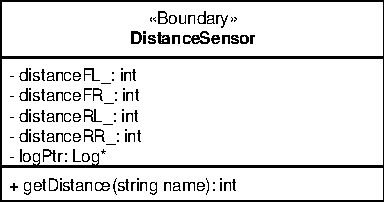
\includegraphics[]{../fig/diagrammer/bil/cd_distancesensor.pdf}
\caption{Klassebeskrivelse af boundary-klassen DistanceSensor}
\label{fig:cd_distancesensor}
\end{figure}

\textbf{Attributter}

\begin{table}[h]
\begin{tabularx}{\textwidth}{| Z | Z | L{10cm} |} \hline
Navn & Type & Beskrivelse \\\hline
\texttt{addrFL} & \texttt{int} &Adresse til forreste venstre afstandssensor.\\\hline
\texttt{addrFR} & \texttt{int} &Adresse til forreste højre afstandssensor.\\\hline
\texttt{addrRL} & \texttt{int} &Adresse til bagerste venstre afstandssensor.\\\hline
\texttt{addrRR} & \texttt{int} &Adresse til bagerste højre afstandssensor.\\\hline
\texttt{distanceFL} & \texttt{int} &Midlertidig variabel der indeholder afstanden fra forreste venstre afstandssensor.\\\hline
\texttt{distanceFR} & \texttt{int} &Midlertidig variabel der indeholder afstanden fra forreste højre afstandssensor.\\\hline
\texttt{distanceRL} & \texttt{int} &Midlertidig variabel der indeholder afstanden fra bagerste venstre afstandssensor.\\\hline
\texttt{distanceRR} & \texttt{int} &Midlertidig variabel der indeholder afstanden fra bagerste højre afstandssensor.\\\hline
\texttt{fd} & \texttt{int} &Variabel der anvendes som reference til i2c-bussen som sensorerne er tilkoblet\\\hline
\texttt{logEntry} & \texttt{string} &Variabel der indeholder reference til loggen.\\\hline
\end{tabularx}
\caption{Attributter for klassen DistanceSensor}
\label{table:attr_distancesensor}
\end{table}

\textbf{Metoder}

\begin{table}[h]
\begin{tabularx}{\textwidth}{| L{2.5 cm} | Z |} \hline
Prototype & \texttt{int getDistance(string name)} \\\hline
Parametre & \texttt{name} \newline Navnet på den sensor som der skal læses fra. Kan en af fire muligheder "FL", "FR", "RL" og "RR". \\\hline
Returværdi &  \texttt{int} \newline Afstanden for til nærmeste sensor for den pågældende sensor. Tallet er angivet i cm. \\\hline
Beskrivelse & Metoden læser afstanden som en afstandssensor befinder sig fra en forhindring. \\\hline
\end{tabularx}
\caption{Metodebeskrivelse for \texttt{getDistance}}
\label{table:met_getdistance}
\end{table}